\chapter{Introdução}        
\label{ch:introducao}
% A atividade de teste é essencial dentro do contexto da Engenharia de Software objetivando a validação do comportamento
% do software e identificação de possíveis problemas de funcionamento. Nas últimas décadas, tem sido estabelecidas
% técnicas, critérios, métodos e ferramentas para a produção de software a fim de acompanhar a crescente utilização de
% sistemas por parte da maioria das práticas da atividade humana~\cite{maldonado2004introduccao}.

% Através da examinação diretamente do software em execução, o teste fornece um \textit{feedback} realista de seu comportamento,
% o que o torna o complemento inevitável de outras técnicas de análise e garantia de qualidade na indústria~\cite{bertolino2007software}.

    \section{Contexto}

O Governo Federal Brasileiro tem incentivado os órgãos públicos a transformarem seus serviços em serviços digitais. Algumas das iniciativas que envolvem este trabalho estão relacionadas à publicação de estratégias e decretos que buscam concretizar o uso de tecnologias digitais como uma estratégia de modernização de determinados setores, como por exemplo, a criação de uma plataforma digital, a criação de um kit para transformação de serviços em serviços digitais e a oferta de uma solução tecnológica para a digitização de serviços. 

Diante do cenário apresentado, a Universidade de Brasília (UnB), por meio do \textit{Information Technology Research and Application Center} (ITRAC), laboratório que promove projetos de pesquisa e desenvolvimento na área de TI, tem contribuído com o ME no apoio ao Kit de Transformação. A parceria entre essas duas instituições relaciona assuntos sobre como colaborar com o Ministério, definindo um processo de transformação de serviços públicos, com a inserção de atividades de qualidade e de desenvolvimento de software.

Em 2017, o MP lançou programa de \textit{Transformação de Serviços Públicos} denominado \textit{Kit de Transformação}, composto de seis fases independentes entre si: \textit{Questione}, \textit{Personalize},\textit{Reinvente}, \textit{Facilite},\textit{Integre} e \textit{Comunique} \cite{BRASIL2017}. O principal objetivo do Kit é simplificar o acesso a determinados serviços e ofertas, a partir da perspectiva dos cidadãos e de empresas.

O presente trabalho está relacionado à fase \textit{Facilite}. Essa fase provê recursos e ferramentas para apoiar os órgãos federais a simplificar e digitizar seus serviços a partir de uma solução tecnológica.

No ITRAC foi definido um processo de digitização de serviços governamentais, que faz uso de uma ferramenta baseada numa abordagem de \textit{meta-design}~\cite{fogli2012meta}, que utiliza modelagem de processos e configuração gráfica dos campos envolvidos para transformação dos serviços governamentais. Esta ferramenta foi adotada pelo ME, via terceirização, e possibilita um processo de desenvolvimento descentralizado que dá celeridade ao processo de transformação digital no governo brasileiro. O processo de transformação envolve o emprego de técnicas que vão desde a análise do serviço, passando por elicitação dos requisitos, mapeamento do processo envolvido no serviço analisado e construção do mesmo na ferramenta de \textit{meta-design}. O processo de transformação envolve, ainda, atividades de Verificação e Validação do serviço digitizado, buscando garantir a qualidade do produto que será entregue a população.

Para o processo de Verificação e Validação dos serviços transformados, as atividades de testes dependem fortemente dos requisitos dos serviços transformados. Contudo, muitas vezes, os requisitos inexistem ou estão instáveis, isto é, os requisitos fornecidos pelos órgãos não são concisos.

A problemática de se testar sem requisitos está presente neste trabalho, visto que os serviços digitizados não possuem uma documentação formal de requisitos e o código-fonte não é acessível à equipe de teste, o que dificulta a extração de informações.

Segundo Barr et. al.,~\cite{barr2015oracle} requisitos instáveis ou inexistentes podem fazer com que os testadores se deparem com o Problema do Oráculo, ou seja, um cenário de difícil identificação do comportamento correto do serviço digitizado, dificultando a comparação entre o comportamento obtido e o comportamento esperado durante a execução dos casos de teste.

No ITRAC, foi desenvolvido um processo de validação sistematizado, com o intuito de garantir a qualidade da digitização dos serviços.  Dado que o código-fonte do serviço não está disponível, o processo emprega a técnica de Teste Exploratório, sugerido por \cite{whittaker2009exploratory}. 

Esta abordagem torna possível que o testador não dependa de um conjunto de casos de teste pré-projetados e utilize da Metáfora do Turista, também proposta por~\cite{whittaker2009exploratory}, como uma estratégia para guiar, através das chamadas \textit{"tours"}, a criação e execução dos casos de teste, facilitando, ainda, a extração de requisitos e regras de negócio a partir da exploração do software analisado.

Vale ressaltar que a utilização dos Testes Exploratórios, com a Metáfora do Turista, dependem da imaginação,  personalidade e conhecimento dos envolvidos na atividade de teste~\cite{itkonen2012role}. Isso se dá, devido ao quesito humano envolvido na atividade de Teste Exploratório, destacado por \cite{whittaker2009exploratory}.

Dessa forma, supõe-se que o perfil do testador tenha algum impacto na aplicação das \textit{tours} utilizadas na metáfora do turista proposta por \cite{whittaker2009exploratory}, visto que os casos de teste gerados e suas sequências variam muito a depender do testador. O entendimento desse perfil e suas principais características pode trazer benefícios para a equipe de testes.

Entre os benefícios envolvidos, podemos destacar a atividade de Atribuição de casos de teste para testadores.
Normalmente, casos de teste são alocados por gerentes para que sejam executados pelos testadores que estiverem disponíveis em determinado momento. Em vista disso, uma das formas de se maximizar a produtividade em uma equipe de testes é alocar casos de teste de acordo com o perfil de testadores~\cite{miranda2012recommender}. Entretanto, a Atribuição de teste manual não é uma tarefa trivial visto que,
em grandes empresas, o gerentes de teste são responsáveis por alocar grandes números de casos de teste para vários testadores.

Neste sentido, sistemas de recomendação têm sido propostos para alocar tarefas a perfis específicos baseado em análises de alocações anteriores, 
como mostram os trabalhos de \cite{anvik2006should} e \cite{miranda2012recommender}. Estes trabalhos impulsionam uma nova utilização de sistemas de recomendação que motiva este trabalho, visto que o desenvolvimento de um sistema de recomendação pode auxiliar na Atribuição de casos de teste para uma equipe de testadores, buscando maximizar a eficiência deles e contribuir com grandes equipes.







% Através do advento da evolução da tecnologia e expansão da internet surge a expressão \textit{Governo Digital},
% que se refere ao uso de tecnologias digitais como uma estratégia de modernização de um Governo, que adota a tecnologia
% da informação e comunicação (TIC) para prover serviços~\cite{fang2002government}. O termo \textit{e-Gov} surgiu no final da década de 1990 e cresceu a um tamanho considerável desde então. Nos últimos
% anos, deu origem a várias conferências de cunho científico, aumentando seu conteúdo e posição no que se refere a outros
% campos de pesquisa e disciplinas~\cite{gronlund2005introducing}.

% No Brasil, embora as medidas de modernização do setor público tenham começado a ser adotadas na década de 70, as ênfases se deram
% apenas com a crise fiscal dos anos 80, onde a intervenção estatal ficou conhecida como reforma da gestão pública que, aliada as
% TICs, proporcionou com que os governos no Brasil oferecessem serviços públicos eletrônicos à população no início da década de
% 2000~\cite{przeybilovicz2015desenvolvimento}.



% Em vista deste cenário de digitalização do serviço público, é de suma importância garantir a qualidade dos serviços digitalizados
% devido aos efeitos nos domínios nacionais e internacionais. De acordo com~\cite{myers2004art}, é preciso que as características
% dos projetos sejam levadas em consideração no momento de definição da estratégia de teste para assegurar que a verificação e
% a validação sejam economicamente viáveis, analisando a complexidade e quantidade de caminhos envolvidos para que se atinja a
% qualidade desejada.






    
    \section{Problema}

A forma como os casos de teste são criados dentro de uma equipe pode implicar na produtividade a depender do nível de expertise dos
testadores. Dentro do presente contexto, sabe-se que a experiência dos testadores relacionados aos serviços disponibilizados
pode variar bastante, devido às variações de nível de escolaridade, experiência com testes, tipos de testes, técnicas já utilizadas
e outras variáveis que serão tratadas mais afundo ao longo deste trabalho.

Por este motivo, a problemática relacionada a estes pontos está relacionada com a produtividade das equipes de teste manual quando voltadas à digitalização de serviços públicos. 

%Há algumas questões de pesquisas relacionadas a este trabalho, que serão abordadas a partir do modelo
%\textit{Goal Question Metric} (GQM), na seção X desse trabalho, especificamente.

Sendo assim, a pergunta de pesquisa definida neste trabalho é:

\textit{``Como maximizar a produtividade de uma equipe de teste manual no contexto de digitalização de serviços públicos?''}

    \section{Objetivos}
\subsection{Objetivo Geral}

Obter perfis de testadores utilizando características pessoais e experiência do domínio para atribuição automática de casos de teste, utilizando a equipe de transformação do ITRAC - Information Technology and Application Center.

\subsection{Objetivos Específicos}

\begin{itemize}
		\item Identificar a interferência que o perfil do testador tem na eficiência dos testes;
		\item Propor uma atribuição automática de casos de teste adequada ao perfil do testador; 
		\item Analisar dados registrados durante os ciclos de teste;
	\end{itemize}



    \section{Metodologia}

É importante que se destaque a classificação de cada escolha metodológica realizada para a configuração deste trabalho. A Figura \ref{fig:classificacaoMetodologica}  apresenta esta classificação.

        \begin{figure}[h]
          \centering
          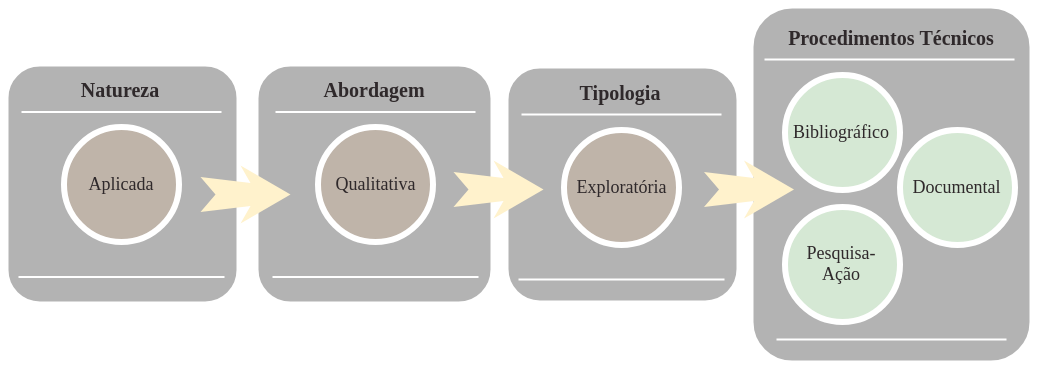
\includegraphics[width=14cm]{figuras/classificacaoMetodologica.png}
          \caption{Classificação Metodológica. (Fonte: Elaborado pela Autora.)} 
          \label{fig:classificacaoMetodologica}
        
        \end{figure}


Dado o contexto prático, no qual o objetivo é a criação de um módulo de uma ferramenta que promoverá a recomendação de \textit{tours} de Teste Exploratório baseado no perfil do testador, esta pesquisa é de natureza aplicada. A abordagem é qualitativa e quantitativa, uma vez que a análise dos dados fará uso de métodos e técnicas estatísticas.

Quanto ao tipo/objetivo, a pesquisa é classificada como explicativa, que possibilita a identificação de fatores que contribuem ou determinam a ocorrência de fenômenos,de modo a aprofundar o conhecimento da realidade e a explicar a razão e motivo das coisas~\cite{gil2002elaborar}. 

Dado que se busca criar um módulo em uma ferramenta, neste trabalho adotou-se a técnica de pesquisa-ação, que possibilita
ao pesquisador a construção de instrumentos em ciclos de iteração com a equipe, isso é, entre os pesquisadores e a organização alvo de estudos. Dessa forma, será possível a construção da ferramenta em ciclos de interação com o refinamento e validação do algoritmo de recomendação de \textit{tours} baseado em cada perfil de testador.

A Pesquisa-ação, proposta por~\cite{petersen2008systematic} é empregad com as etapas Diagnóstico, Planejamento da ação, Reflexão e Tomada de decisão, cujo objetivo é a realização de ciclos de iteração para a especificação de um instrumento; seguida da técnica Estudo de Caso empregada na Construção do instrumento, cujo objetivo é desenvolver um sistema a partir da especificação definida de forma iterativa na fase anterior, como demonstrado na Figura \ref{fig:etapasPesquisaAcaoAdotas}.

        \begin{figure}[H]
          \centering
          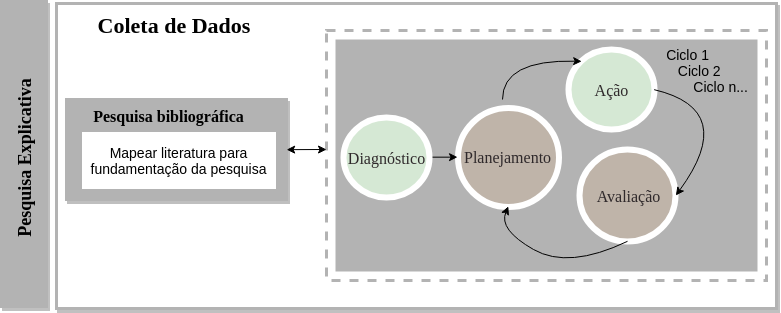
\includegraphics[width=12cm]{figuras/etapasPesquisaAcaoAdotadas.png}
          \caption{Etapas da Pesquisa-Ação adotadas. (Fonte: Elaborado pela Autora.)} 
          \label{fig:etapasPesquisaAcaoAdotas}
        
        \end{figure}

O plano metodológico adotado neste trabalho compreendeu quatro fases básicas: \textit{planejamento da pesquisa}; \textit{coleta de dados}; \textit{análise dos dados}; e \textit{relato dos resultados}. O detalhamento deste planejamento metodológico encontra-se no Capítulo Materiais e Métodos.




    \section{Organização do Trabalho}

Este trabalho de conclusão de curso está organizado nos seguintes capítulos:

\begin{itemize}
    \item \textbf{Capítulo \ref{ch:introducao} - Introdução:} apresenta Contextualização, justificativa, problema de pesquisa, justificativa e objetivos;
    \item \textbf{Capítulo \ref{ch:referencial} - Referencial teórico:} descreve os conceitos que fundamentam o trabalho reunindo conhecimento necessário para que se compreenda a pesquisa realizada. O capítulo é subdividido nas seções \textit{Governo Digital}, \textit{Testes Exploratórios} e \textit{Sistema de Recomendação};
    % \item \textbf{Capítulo \ref{ch:suporte} - Suporte tecnológico:} apresenta as ferramentas que suportarão as atividades de desenvolvimento de software, gerenciamento, documentação, dentre outras.
     \item \textbf{Capítulo \ref{ch:metodologia} - Materiais e Métodos:} apresenta o plano metodológico adotado e caracteriza o objeto e estudo;
     \item \textbf{Capítulo \ref{ch:proposta} - Proposta:} Apresenta a proposta deste trabalho, desde a abordagem proposta até a proposta de um módulo para a ferramenta de suporte ao processo de transformação digital do governo brasileiro.
     
    % \item \textbf{Capítulo \ref{ch:resultados} - Resultados parciais:} apresenta os resultados alcançados durante o TCC1.
    
    % \item \textbf{Capítulo \ref{ch:consideracoes} - Considerações finais:} relata o status do trabalho alcançado até a execução do TCC1 e os resultados esperados para o TCC2.
\end{itemize}
